\documentclass[twocolumn]{IEEEtran}
\usepackage{graphicx}
\usepackage[utf8x]{inputenc}
\usepackage{times}
\usepackage{amssymb,amsfonts}
\usepackage{pict2e}
\usepackage{float}
\usepackage[all]{xy}
\usepackage{graphics,graphicx,color,colortbl}
\usepackage{subfigure}
\usepackage{wrapfig}
\usepackage{multicol}
\usepackage{cite}
\usepackage{url}
\usepackage[tbtags]{amsmath}
\usepackage{amsmath,amssymb,amsfonts,amsbsy}
\usepackage{bm}
\usepackage{listings}
\usepackage{algorithm}
\usepackage{algorithmic}
\usepackage[centerlast, small]{caption}
\usepackage[colorlinks=true, citecolor=blue, linkcolor=blue, urlcolor=blue, breaklinks=true]{hyperref}
\hyphenation{ele-men-tos he-rra-mi-en-ta cons-tru-yen trans-fe-ren-ci-a}

\begin{document}
\title{Control ON/OFF y Control Proporcional}
\author{Israel Ricardo Bernal Sánchez Código: $261613$\\
	Felipe Castañeda Prieto Código $285728$\\
	David Ricardo Martínez Hernández Código: $261931$\\
	Oscar Andrés Urbano Vallejo Código: $261683$}
\maketitle
\markboth{Universidad Nacional de Colombia}{}
\floatname{algorithm}{Algoritmo}

\begin{abstract}

\end{abstract}

\begin{keywords}
 
\end{keywords}

\section{Introducción}


\section{Procedimiento}
\subsection{Control ON/OFF del motor LEGO}
\noindent



\subsection{Control Proporcional del Motor LEGO}
\noindent

\subsubsection{Punto 4.2.3}
\noindent
Dada la función de transferencia $G(s)=\frac{8.181818}{0.061s+1}$, siendo la constante de tiempo $\tau=0.061$, el polo se encuentra situado en $s=-\frac{1}{\tau}$. Dado que es necesario estabilizar el sistema en lazo cerrado $2$ veces más rápido que en lazo abierto, el valor de la ganancia $K_p$ (controlador) fue el siguiente:
$$ 2\tau=0.061 \rightarrow \tau=\frac{0.061}{2} $$
\noindent
evaluando el nuevo valor de $\tau$ en la función de Transferencia
\begin{equation}
 G(s)=\frac{8.181818}{\frac{0.061}{2}s+1}
\label{ecu1}
\end{equation}
\noindent
Como es necesario calcular la función de transferencia en lazo cerrado se llego a que la ecuación general es
$$ G_{LC} \left( s \right) = \frac{{K_p G\left( s \right) }}{{1 + K_p G\left( s \right) }} $$
\noindent
reemplazando los valores de $G\left( s \right)$ se obtuvo lo siguiente
\begin{equation}
 G_{LC} \left( s \right) = \frac{{8.181818 K_p }}{{0.061s + 8.181818 K_p + 1}}
\label{ecu2}
\end{equation}
\noindent
se despejo del polinomio característico $\Delta\left( s \right)=0.061s + 8.181818 K_p + 1$ evaluando en $s=0$, el valor de $K_p$ es:
\begin{equation*}
 K_p=\frac{1}{8.181818}\approx 0.122222224938272
\end{equation*}
\begin{figure}[H]
	\centering
		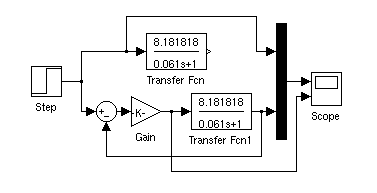
\includegraphics[scale=1]{figure1.png}
	\caption{Diagrama de Bloques en Simulink}
	\label{fig1}
\end{figure}
\begin{figure}[H]
	\centering
		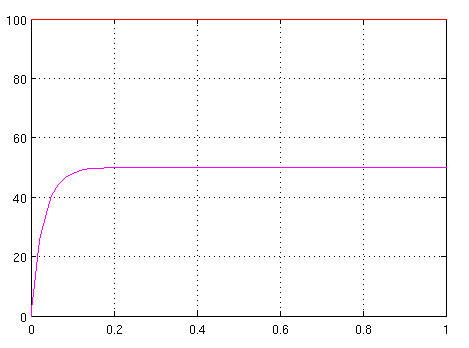
\includegraphics[scale=0.8]{salida1.png}
	\caption{Salida teórica se Simulink}
	\label{fig2}
\end{figure}

\subsubsection{Punto 4.2.4}
\noindent
Con la función de transferencia anterior ecu. (\ref{ecu2}), se requiere que tenga un error permanate del $10\%$
\begin{equation*}
 \frac{{Y\left( 0 \right)}}{{U\left( 0 \right)}} = \frac{{8.181818K_p }}{{0.061s + 8.181818s + 1}}
\end{equation*}
\begin{equation*}
\frac{{90}}{{100}} = \frac{{8.181818K_p }}{{0.061s + 8.181818K_p  + 1}} 
\end{equation*}
\noindent
Despejando el valor de $K_p$ se obtiene:
\begin{equation*}
 K_p  = \frac{{\frac{{90}}{{100}}}}{{8.181818\left( {1 - \frac{{90}}{{100}}} \right)}}\approx 1.10000002444445
\end{equation*}
\begin{figure}[H]
	\centering
		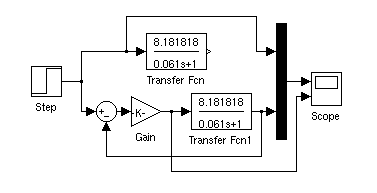
\includegraphics[scale=1]{figure1.png}
	\caption{Diagrama de Bloques en Simulink}
	\label{fig3}
\end{figure}
\begin{figure}[H]
	\centering
		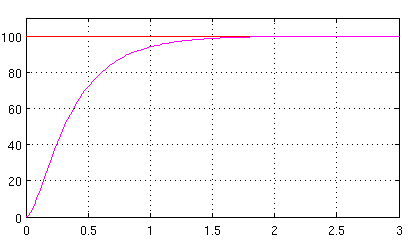
\includegraphics[scale=0.85]{salida2.png}
	\caption{Salida teórica se Simulink}
	\label{fig4}
\end{figure}

\subsubsection{Punto 4.2.4}
\noindent

\section{Conclusiones}
\begin{itemize}
 \item .
 \item .
 \item .
\end{itemize}

\bibliographystyle{ieeetran}
\begin{thebibliography}{99}

\bibitem{chen} Chen, Chi-Tsong.
{\em "`Analog and Digital Control System Desing: Transfer-Function, State, Space and Algebraic Methods"'}.
Saunders College Publishing, 1993.

\bibitem{kuo} Kuo, C. Benjamin.
{\em "`Sistemas Automáticos de Control"'}.
Pentice Hall Hispanoamerica, Séptima Edición, 1996.

\bibitem{ogata} Ogata, Katsuhiko.
{\em "`Ingeniería De Control Moderna"'}.
Pearson Educación, Tercera Edición, 1998.

\end{thebibliography}
\end{document}